%%%%%%%%%%%%%%%%%%%%%%%%%%%%%%%%%%%%%%%%%%%%%%%%%%%%%%%%
%%%%                                              %%%%%%
%%%%  Author: Peter Wilson                        %%%%%%
%%%%                                              %%%%%%
%%%%  ANDES quad element                          %%%%%%
%%%%                                              %%%%%%
%%%%%%%%%%%%%%%%%%%%%%%%%%%%%%%%%%%%%%%%%%%%%%%%%%%%%%%%


%fref generates automatically the respective abreviation/word in the text for the reference. You just have to define a label starting with the respective keyword.
%english: chap, sec, fig, eq, app
%deutsch: chap/kap, abs, abb, gl, anh
%see http://ctan.space-pro.be/tex-archive/macros/latex/contrib/fancyref/fancyref.pdf for more information

\renewcommand{\Thema}{Benchmarking}



\chapter{Benchmarking}

Benchmarking yeah

\section{Nonlinear benchmarks}

asdfasdf

\subsection{Hinged cylindrical roof}

\begin{figure}[H]
	\centering
	\def\svgwidth{\columnwidth}
	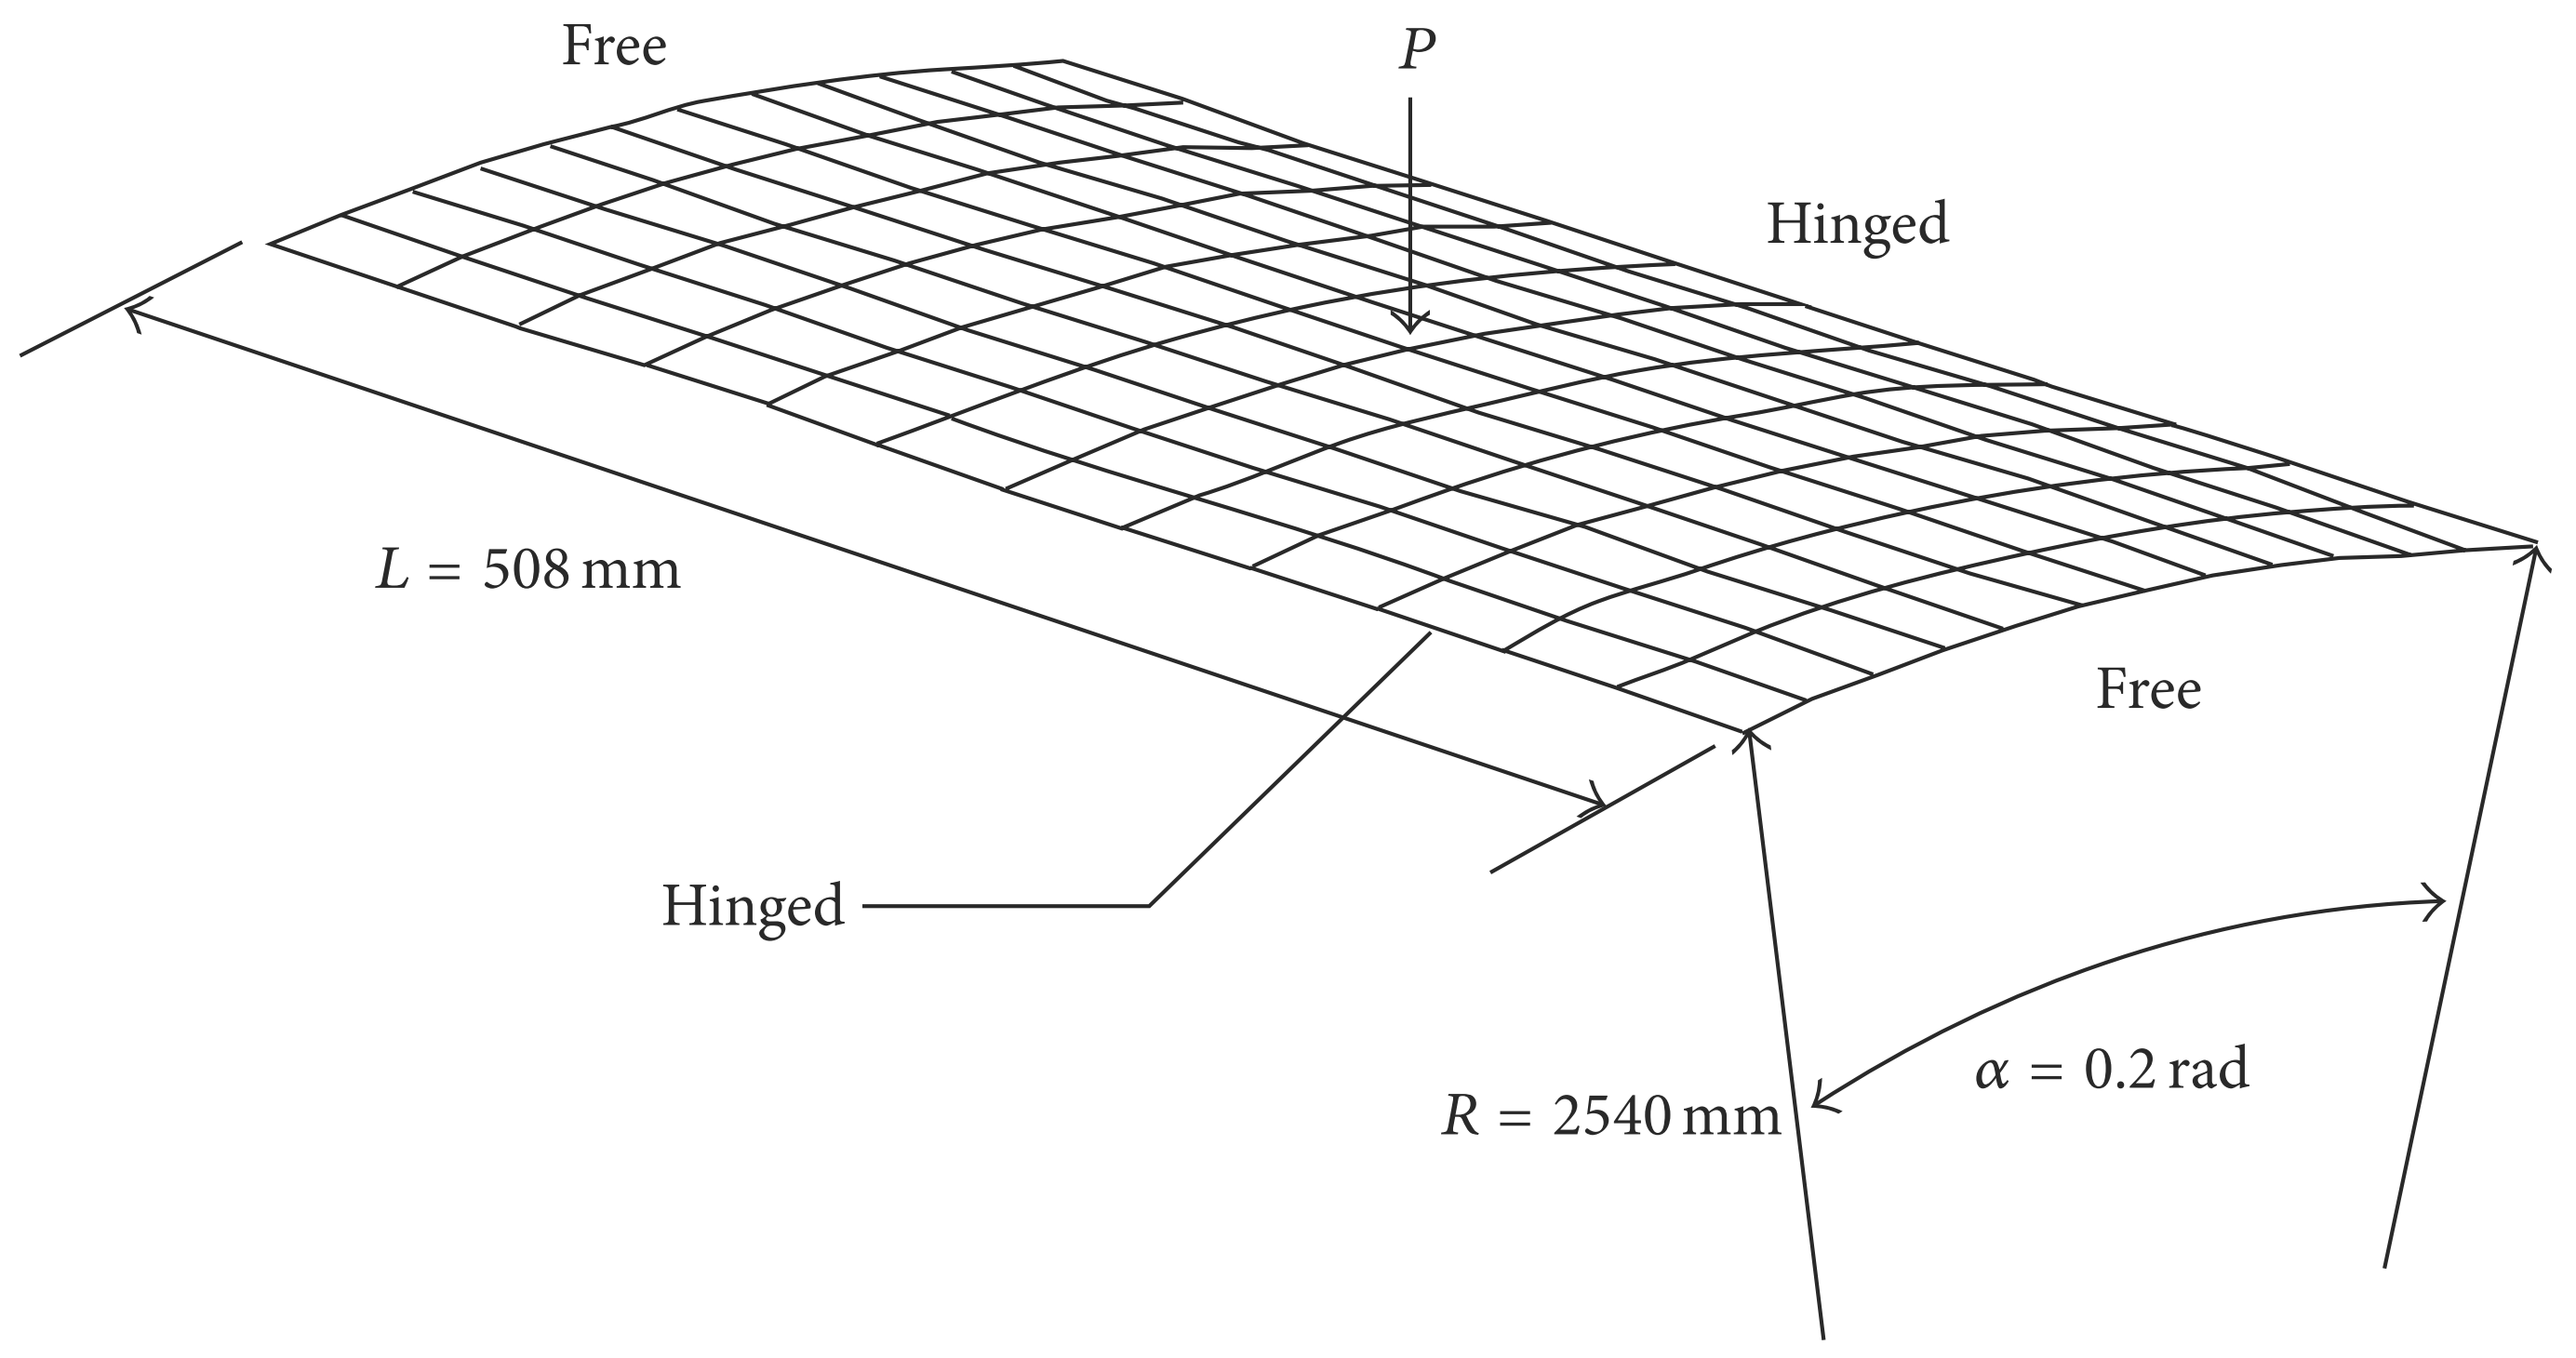
\includegraphics[width=12cm]{images/hinged_cylindrical_roof.png}
	\caption{Problem definition of the hinged cylindrical roof benchmark \cite{Jung13}}
	\label{benchmark_hinged_cylindrical_roof}
\end{figure}

asdfasdf

\begin{figure}[H]
	\centering
	\def\svgwidth{\columnwidth}
	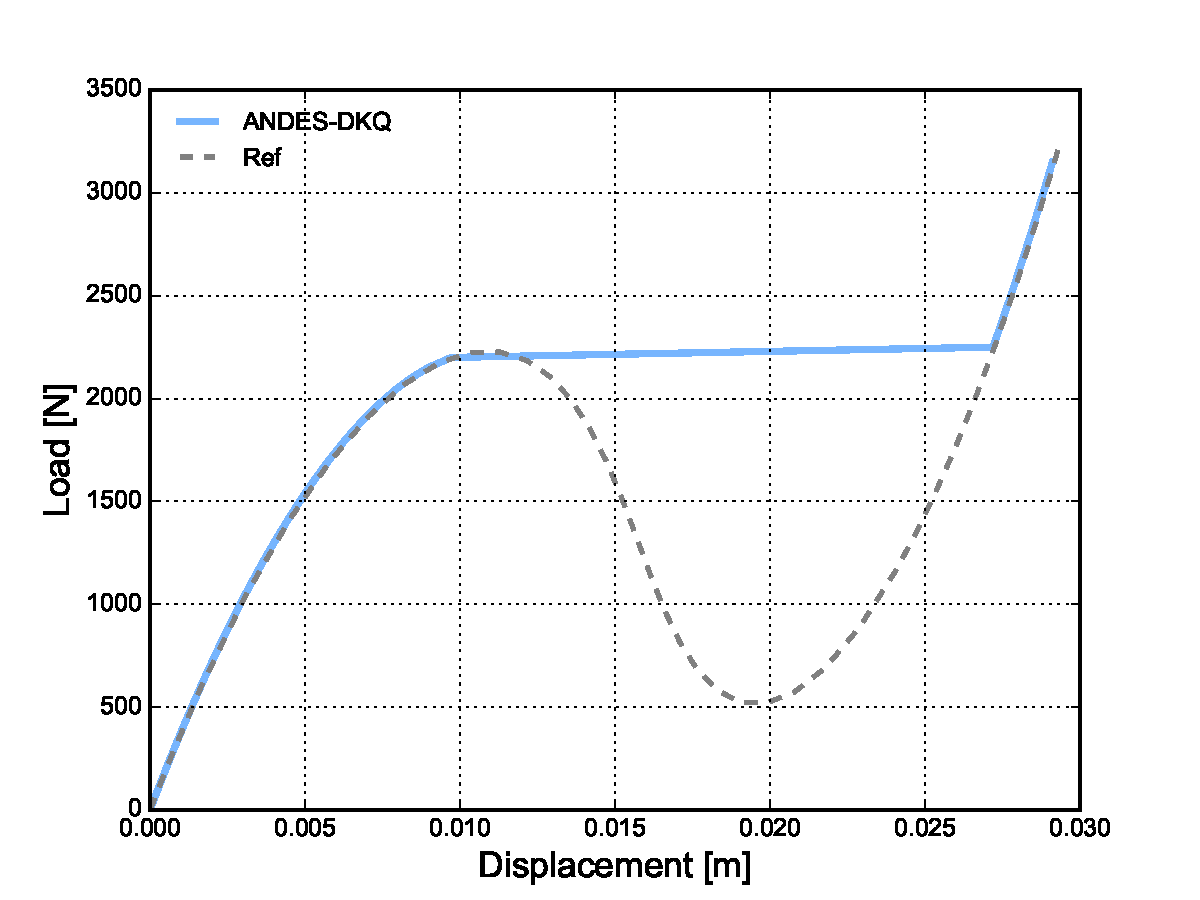
\includegraphics[width=12cm]{images/Load_displacement_curve_hinged_cylindrical_roof.pdf}
	\caption{Load-displacement curve of hinged cylindrical roof}
	\label{benchmark_hinged_cylindrical_roof}
\end{figure}

reference solution from \cite{Sze2004}

sadf